
% \iffalse meta-comment
%
% Copyright (C) 2011 by Enrico Jörns
% -----------------------------------
%
% This file may be distributed and/or modified under the
% conditions of the LaTeX Project Public License, either version 1.2
% of this license or (at your option) any later version.
% The latest version of this license is in:
%
%   http://www.latex-project.org/lppl.txt
%
% and version 1.2 or later is part of all distributions of LaTeX
% version 1999/12/01 or later.
%
% \fi
%
% \CheckSum{0}
%
% \CharacterTable
%  {Upper-case    \A\B\C\D\E\F\G\H\I\J\K\L\M\N\O\P\Q\R\S\T\U\V\W\X\Y\Z
%   Lower-case    \a\b\c\d\e\f\g\h\i\j\k\l\m\n\o\p\q\r\s\t\u\v\w\x\y\z
%   Digits        \0\1\2\3\4\5\6\7\8\9
%   Exclamation   \!     Double quote  \"     Hash (number) \#
%   Dollar        \$     Percent       \%     Ampersand     \&
%   Acute accent  \'     Left paren    \(     Right paren   \)
%   Asterisk      \*     Plus          \+     Comma         \,
%   Minus         \-     Point         \.     Solidus       \/
%   Colon         \:     Semicolon     \;     Less than     \<
%   Equals        \=     Greater than  \>     Question mark \?
%   Commercial at \@     Left bracket  \[     Backslash     \\
%   Right bracket \]     Circumflex    \^     Underscore    \_
%   Grave accent  \`     Left brace    \{     Vertical bar  \|
%   Right brace   \}     Tilde         \~}
%
% \iffalse
%
%<*driver>
\documentclass{ltxdoc}
\usepackage[ngerman]{babel}
\usepackage[utf8]{inputenc}
\usepackage{nexus}
\usepackage[colorlinks, linkcolor=blue]{hyperref}
\usepackage{tabularx}
\EnableCrossrefs
\CodelineIndex
\RecordChanges
\begin{document}
  \DocInput{tubsbox.dtx}
\end{document}
%</driver>
% \fi
%
% \newenvironment{key}[2]{\expandafter\macro\expandafter{`#2'}}{\endmacro}
% \newenvironment{Options}%
%  {\begin{list}{}{%
%   \renewcommand{\makelabel}[1]{\texttt{##1}\hfil}%
%   \setlength{\itemsep}{-.5\parsep}
%   \settowidth{\labelwidth}{\texttt{xxxxxxxxxxx\space}}%
%   \setlength{\leftmargin}{\labelwidth}%
%   \addtolength{\leftmargin}{\labelsep}}%
%   \raggedright}
%  {\end{list}}
%
% \changes{v1.0}{ 2011 / 08 / 23 }{Initial version}
% \changes{v1.1}{ 2011 / 08 / 23 }{%
%   Fehler bei Darstellung von modsubrow am Zeilenende behoben,
%   Hintergrundfarbe als Option nutzbar
% }
%
% \GetFileInfo{tubsbox.sty}
%
% \DoNotIndex{ list of control sequences }
%
% \title{\textsf{tubsbox} -- 
%   Box-Definitionen für \emph{tubslatex}\thanks{This document
%   corresponds to \textsf{tubsbox}~\fileversion,
%   dated \filedate.}}
% \author{Enrico Jörns \\ \texttt{e dot joerns at tu minus bs dot de}}
%
% \maketitle
%
% \begin{abstract}
%   Diese Datei stellt die Umgebung |gaussbox| für Darstellungen im Gaußraster 
%   und Umgebungen für Darstellungen im Modulraster zur Verfügung.
% \end{abstract}
%
% \tableofcontents
%
% \section{Benutzung}
%
% \subsection{Gaußraster}
%
% Das Gaußraster wird zur Inhalts-Darstellung auf Postern und Titelseiten 
% verwendet.
%
% \DescribeEnv{gaussbox} Box im Gauß-Raster
%
% Syntax: |\gaussbox|\oarg{options}\marg{}
%
%
% \subsection{Modulsystem}
%
% Das Modulsystem wird ausschließlich für wissenschaftliche Plakate verwendet.
%
% \StopEventually{\PrintIndex}
%
% \section{Implementierung}
%
%
%    \begin{macrocode}
%<*package>
%    \end{macrocode}
%
% Es werden die folgenden Pakete geladen: |ifthen| und |xkeyval| werden
% allgemein zum Definieren und Auswerten von Optionen etc. benötigt.
% |etoolbox| und |forloop| werden für die Auswertung von kommagetrennten
% Listen benutzt. Aus |tubstypearea| werden alle benötigten Längen entnommen,
% um die Boxen mit |texpos| korrekt positionieren zu können.
%    \begin{macrocode}
\RequirePackage{ifthen}
\RequirePackage{xkeyval}
\RequirePackage{etoolbox}
\RequirePackage{forloop}
\RequirePackage{tubstypearea}
\RequirePackage[absolute]{textpos}
%    \end{macrocode}
%
% \subsection{Allgemeine Optionen / Paketoptionen}\label{sec:options}
%
%    \begin{macro}{tubsbox@bottomsender}
% Merker für Option '|sender|'.
%    \begin{macrocode}
\newboolean{tubsbox@bottomsender}\setboolean{tubsbox@bottomsender}{false}
%    \end{macrocode}
%    \end{macro}
%
%    \begin{macro}{\tubsbox@framebox}
% Speichert ggf. Kommando mit dem ein Rahmen um die jeweilige Box
% gezeichnet werden soll.
%    \begin{macrocode}
\def\tubsbox@framebox{\relax}
%    \end{macrocode}
%    \end{macro}
%
%    \begin{macro}{\tubsbox@colorbox}
% Speichert ggf. colorbox-Kommand mit dem die Hintergrundfarbe der jeweiligen
% Box gezeichnet werden soll.
%    \begin{macrocode}
\newcommand{\tubsbox@colorbox}{\relax}
%    \end{macrocode}
%    \end{macro}
%
%    \begin{macro}{\if@tubs@oddpage}
% \marg{odd cmd}\marg{even cmd}\par
% Switch um Kommandos zu definieren, die für gerade und ungerade Seiten
% unterschiedlich arbeiten.
% Ist nur aktiv, wenn Option |twosided| benutzt wird.
%    \begin{macrocode}
\newcommand{\if@tubs@oddpage}[2]{%
  \ifthenelse{\boolean{tubsstyle@twoside}}{%
    \ifthispageodd{#1}{#2}%
  }{#1}%
}
%    \end{macrocode}
%    \end{macro}
%
%
%    \begin{macro}{\tubsboxsetup}
%    \begin{macro}{\gaussboxsetup}
%    \begin{macro}{\scifiboxsetup}
% \oarg{option}\par
% Aktualisiert alle durch Optionen übergebenen Einstellungen an den Boxen.
% Die Namen sind jeweils Aliase.
%    \begin{macrocode}
\newcommand{\tubsboxsetup}[1][]{%
  \setkeys{tubsbox.sty}{#1}
}
\let\gaussboxsetup=\tubsboxsetup%
\let\scifiboxsetup=\tubsboxsetup%
%    \end{macrocode}
%    \end{macro}\end{macro}\end{macro}
%
%
% \begin{key}{tubsbox.sty}{sender}
% Mögliche Werte: |bottom| oder |top|.
% Schaltet zwischen den beiden Layoutvarianten mit Absenderbereich oben
% und unten auf der Seite um, damit die Boxen korrekt platziert werden.\par
% Standardmäßig ist der Absenderbereich oben.
%    \begin{macrocode}
\define@choicekey{tubsbox.sty}{sender}[\var\nr]{top,bottom}{%
  \ifcase\nr\relax
    \setboolean{tubsbox@bottomsender}{false}
  \or
    \setboolean{tubsbox@bottomsender}{true}
  \fi
}
%    \end{macrocode}
%    \end{key}
%
% \begin{key}{tubsbox.sty}{frame}
%   Zeichnet wenn gewünscht einen Rahmen um
%   die jeweiligen Boxen.
%   Mögliche Werte: |none| - Kein Rahmen, |fbox| - einfacher Rahmen.\par
%   Standardmäßig haben die Boxen keinen Rahmen.
%    \begin{macrocode}
\define@choicekey{tubsbox.sty}{frame}[\val\nr]{none,fbox}{%
  \ifcase\nr\relax
    \def\tubsbox@framebox{\relax}
  \or
    \def\tubsbox@framebox{\fbox}
  \fi
}
%    \end{macrocode}
%    \end{key}
%
% \begin{key}{tubsbox.sty}{bgcolor}
%   Standard-Hintergrundfarbe der Boxen festlegen.
%   Mögliche Werte sind |none|, sowie die jeweilige gewünschte Farbe.\par
%   Standardmäßig haben die Boxen keine Hintergrundfarbe.
%    \begin{macrocode}
\define@key{tubsbox.sty}{bgcolor}{%
  \ifthenelse{\equal{#1}{none}}{%
    \renewcommand\tubsbox@colorbox{\relax}
  }{%
    \def\bgcolor{#1}
    \renewcommand\tubsbox@colorbox{\colorbox{\bgcolor}}
  }
}
%    \end{macrocode}
%    \end{key}
%
%
% Paket-Optionen auswerten,
% Initialisierung mit Werten der Paket-Optionen.
%    \begin{macrocode}
\ProcessOptionsX\relax%
\gaussboxsetup
%    \end{macrocode}%
%
%
% \subsection{Gaussbox-Optionen}
%
%
% \begin{key}{tubsbox.sty}{addtopsep}
% Fügt zusätzlichen Top-Innenabstand hinzu. Wenn kein Wert angegeben, wird
% doppelte Rahmenstärke hinzugefügt. (Dies ist die Standardeinstellung für
% die erste tubsbox auf einer Seite mit Siegelbandlogo.)
%    \begin{macrocode}
\newcommand*\tubs@gb@topsep{0mm}
\define@boolkey{gaussbox}{logosep}[true]{%
  \ifKV@gaussbox@logosep%
    \renewcommand*\tubs@gb@topsep{2\tubspage@borderwidth}
  \else%
    \renewcommand*\tubs@gb@topsep{0mm}
  \fi%
}
%    \end{macrocode}
%    \end{key}
%
%
% \begin{key}{tubsbox.sty}{margin}
%   \emph{TODO}\par
%   Führt dazu, dass \emph{innerhalb} der gaussbox ein zusätzlicher Rand
%   in Breite der Marginale eingefügt wird.
%    \begin{macrocode}
\define@choicekey{gaussbox}{margin}[\val\nr]{left,right,both}{%
  \PackageError{tubsbox}{Option 'margin' is not yet supported}{}
  \ifcase\nr\relax
    %TODO
  \or
    %TODO
  \or
    %TODO
  \fi
}
%    \end{macrocode}
%    \end{key}
%
%
%
%    \begin{macro}{\tubs@gb@setorig}
% Berechnet den Ursprung des von den Boxen benutzten Koordinatensystems neu.
% |\oddsidemargin|+1in+|\voffst| ist der Abstand vom linken Rand!
%    \begin{macrocode}
\providecommand\tubs@gb@setorig{%
  % TODO: this seems to be a bug, only one borderwidth should be needed
  \ifthenelse{\boolean{tubsbox@bottomsender}}{%
    \if@tubs@oddpage{%
      \textblockorigin{2\tubspage@borderwidth+\tubspage@bcor}{%
        2\tubspage@borderwidth}%
    }{%
      \textblockorigin{2\tubspage@borderwidth}{%
        2\tubspage@borderwidth}%
    }%
  }{% 
    \if@tubs@oddpage{%
      \textblockorigin{2\tubspage@borderwidth+\tubspage@bcor}{%
        \tubspage@senderheight+\tubspage@borderwidth}%
    }{%
      \textblockorigin{2\tubspage@borderwidth}{%
        \tubspage@senderheight+\tubspage@borderwidth}%
    }
  }
}
%    \end{macrocode}
%    \end{macro}
%
%
%
%%%%%%%%%%%%%%%%%%%%%%%%%%%%%%%%%%%%%%%%%%%%%%%%%%%%%%%%%%%%%%%%%%%%%%%%%%%%%%%%
% \subsection{Gaußraster-Box}
%%%%%%%%%%%%%%%%%%%%%%%%%%%%%%%%%%%%%%%%%%%%%%%%%%%%%%%%%%%%%%%%%%%%%%%%%%%%%%%%
%
%
% Lege Rastermaße fest.
%    \begin{macrocode}
\setlength{\TPHorizModule}{%
  (\paperwidth-4\tubspage@borderwidth-\tubspage@bcor)*\ratio{1mm}{\tubspage@xsegments mm}}
\setlength{\TPVertModule}{%
  (\tubspage@communicationheight)*\ratio{1mm}{\value{tubspage@gausssum} mm}}
%    \end{macrocode}
%
%    \begin{macro}{\tubs@gb@leftmargin}
%    \begin{macro}{\tubs@gb@rightmargin}
% Korrektur der Textränder links und rechts außen.
%    \begin{macrocode}
\newlength{\tubs@gb@leftmargin}
\newlength{\tubs@gb@rightmargin}
%    \end{macrocode}
%    \end{macro}\end{macro}
%    \begin{macro}{\tubs@gb@leftsep}
%    \begin{macro}{\tubs@gb@rightsep}
%    \begin{macro}{\tubs@gb@topmargin}
%    \begin{macro}{\tubs@gb@toppadding}
% Definition einiger benötigter Längen
%    \begin{macrocode}
\newlength{\tubs@gb@leftsep}
\newlength{\tubs@gb@rightsep}
\newlength{\tubs@gb@topmargin}
\newlength{\tubs@gb@toppadding}
\newlength{\tubs@gb@bottommargin}
%    \end{macrocode}
%    \end{macro}\end{macro}\end{macro}\end{macro}
%
%    \begin{macro}{\tubs@gb@storebox}
% Savebox zum Speichern der Box-Inhalte.
%    \begin{macrocode}
\newsavebox{\tubs@gb@storebox}
%    \end{macrocode}
%    \end{macro}
%
%    \begin{macro}{tubs@gb@lastelement}
%    \begin{macro}{tubs@gb@calcypos}
%    \begin{macro}{tubs@gb@calcheight}
% Definition einiger benötigter Counter.
%    \begin{macrocode}
\newcounter{tubs@gb@lastelement}
\newcounter{tubs@gb@calcypos}
\newcounter{tubs@gb@calcheight}
%    \end{macrocode}
%    \end{macro}\end{macro}\end{macro}
%
%    \begin{macro}{gaussbox}
% \oarg{options}\marg{xpos}\marg{ypos}\marg{widht}\marg{height}\par
% \begin{tabularx}{\textwidth}{lX}
%   |options| & Siehe Abschnit \ref{sec:options}  \\
%   |xpos|    & Horizontaler Startpunt der Box,
%               gemessen im Spalten-Raster,
%               Standard-Wertebereich: [1-6]  \\
%   |ypos|    & Vertikaler Startpunkt der Box,
%               gemessen im Gauß-Raster
%               Standard-Wertebereich: [1-6] (Querformat), [1-8] (Hochformat)\\
%   |width|   & Breite der Box in Spalten,
%               Wertebereich: [1-6] \\
%   |height|  & Höhre der Box in Gaußraster-Elementen,
%               Wertebereich: [1-6] / [1-8]
% \end{tabularx}
%    \begin{macrocode}
\newenvironment{gaussbox}[5][bgcolor=none]{%
\setkeys*{tubsbox.sty}{#1}
\tubs@gb@setorig
\setkeys*{gaussbox}{bgcolor=none,logosep=false,#1}
%    \end{macrocode}
% Berechnung der linken und rechten Ränder
%    \begin{macrocode}
% Berechne Positionen
\ifnum#2=1
\setlength{\tubs@gb@leftmargin}{\tubspage@borderwidth}
\setlength{\tubs@gb@rightmargin}{0mm}
\setlength{\tubs@gb@leftsep}{0mm}
\else
\setlength{\tubs@gb@leftsep}{0.5\tubspage@columnsep}
\fi
%
\setcounter{tubs@gb@lastelement}{#2-1}
\edef\tubs@gb@xpos{\thetubs@gb@lastelement}%TODO: etwas unschön...
\addtocounter{tubs@gb@lastelement}{#4}
\ifnum\value{tubs@gb@lastelement}=\tubspage@xsegments
  \setlength{\tubs@gb@rightmargin}{\tubspage@borderwidth}
  \setlength{\tubs@gb@rightsep}{0mm}
\else
  \setlength{\tubs@gb@rightmargin}{0mm}
  \setlength{\tubs@gb@rightsep}{0.5\tubspage@columnsep}
\fi
%    \end{macrocode}
% Berechnung der oberen und unteren Ränder
%    \begin{macrocode}
\ifnum#3=1
  \setlength{\tubs@gb@topmargin}{\tubspage@borderwidth}
  \setlength{\tubs@gb@toppadding}{\tubspage@borderwidth}
  \addtolength\tubs@gb@toppadding\tubs@gb@topsep
  \setlength{\tubs@gb@bottommargin}{0mm}
\else
  \setlength{\tubs@gb@toppadding}{\tubspage@borderwidth}
\fi
\setcounter{tubs@gb@lastelement}{#3+#5-1}
% Prüfe, ob Werte korrekt
\ifnum\value{tubs@gb@lastelement}>\tubspage@ysegments%
  \PackageError{tubstypearea}{Invalid segment number}{}%
\fi%
\ifnum\value{tubs@gb@lastelement}=\tubspage@ysegments
  \setlength{\tubs@gb@bottommargin}{\tubspage@borderwidth}
\else
  \setlength{\tubs@gb@bottommargin}{0mm}
\fi%


%
% Makro |\@inv@arg| wird benutzt, um Argument 'inverted' zu übergeben
\def\@inv@arg{\relax}
\ifthenelse{\boolean{tubsbox@bottomsender}}{%
  \def\@inv@arg{inverted}%
}{}
\calc@gauss@elementpos[\@inv@arg]{tubs@gb@calcypos}{#3}
\def\tubs@gb@ypos{\thetubs@gb@calcypos}
% 
\calc@gauss@elementpos[\@inv@arg]{tubs@gb@calcheight}{#3+#5}
\addtocounter{tubs@gb@calcheight}{-\thetubs@gb@calcypos}%
% 
\def\tubs@gb@width{#4}%
\def\tubs@gb@height{\thetubs@gb@calcheight}%
\begin{lrbox}{\tubs@gb@storebox}%
\begin{minipage}%
        [t]%
        [\tubs@gb@height\TPVertModule]%
        {\tubs@gb@width\TPHorizModule-\tubs@gb@leftsep-\tubs@gb@rightsep-0.3mm}%
  \vspace*{\tubs@gb@toppadding}%
}{%
  \vspace*{\tubspage@borderwidth}%
  \end{minipage}
  \end{lrbox}
  \setlength{\fboxsep}{0cm}%
  \begin{textblock}{\tubs@gb@width}(\tubs@gb@xpos,\tubs@gb@ypos)%
  \begin{addmargin*}[-\tubs@gb@leftmargin]{-\tubs@gb@rightmargin}%
    \noindent\hspace*{\tubs@gb@leftsep}%
    \raisebox{\tubspage@borderwidth}[0cm]{%
      \tubsbox@framebox{\tubsbox@colorbox{%
        \hspace*{\tubs@gb@leftmargin}%
        \usebox{\tubs@gb@storebox}%
        \hspace*{\tubs@gb@rightmargin}%
        }}%
      }%
  \end{addmargin*}%
  \end{textblock}
}
%    \end{macrocode}
%    \end{macro}
%
% NOTE: Nur aus Kompatibilitaetsgründen definiert!
% Sobald wie möglich entfernen!
%    \begin{macrocode}
\let\tubsbox=\gaussbox
\let\endtubsbox=\endgaussbox
%    \end{macrocode}
%
%
%%%%%%%%%%%%%%%%%%%%%%%%%%%%%%%%%%%%%%%%%%%%%%%%%%%%%%%%%%%%%%%%%%%%%%%%%%%%%%%%
% \subsection{Modul-System}
%%%%%%%%%%%%%%%%%%%%%%%%%%%%%%%%%%%%%%%%%%%%%%%%%%%%%%%%%%%%%%%%%%%%%%%%%%%%%%%%
%
%
%    \begin{macrocode}
\newsavebox{\tubs@sb@storebox}
%    \end{macrocode}
%
%    \begin{macrocode}
\newsavebox{\tubs@sb@bgimagebox}
%    \end{macrocode}
%
%    \begin{macro}{tubs@sb@elementcount}
% Counter zählt Anzahl Zeilen für Box-Layout.
%    \begin{macrocode}
\newcounter{tubs@sb@elementcount}
%    \end{macrocode}
%    \end{macro}
%
%    \begin{macro}{tubs@sb@xcount}
% Counter zählt Anzahl Xen
%    \begin{macrocode}
\newcounter{tubs@sb@xcount}
%    \end{macrocode}
%    \end{macro}
%
%    \begin{macro}{\tubs@sb@xfreespace}
% Länge speichert aktuellen freien Platz für Xe
%    \begin{macrocode}
\newlength{\tubs@sb@xfreespace}
%    \end{macrocode}
%    \end{macro}
%
%    \begin{macro}{\tubs@sb@xlength}
% Länge eines X-Elements
%    \begin{macrocode}
\newlength{\tubs@sb@xlength}
%    \end{macrocode}
%    \end{macro}
%
%    \begin{macro}{tubs@cnt}
% Counter für forloop-Schleife
%    \begin{macrocode}
\newcounter{tubs@cnt}
%    \end{macrocode}
%    \end{macro}
%
% Boolean für Hintergrundbild
%    \begin{macrocode}
\newboolean{scifibox@showbgimage}
%    \end{macrocode}
%
%
%    \begin{key}{scifibox}{bgimage}
%    \begin{macrocode}
\define@key{scifibox}{bgimage}{%
  
}
%    \end{macrocode}
%    \end{key}
%
%
%    \begin{key}{scifibox}{imagefit}
%    \begin{macrocode}
\define@choicekey{scifibox}{imagefit}[\val\nr]{%
        default,scaled,cropped,cropx,cropy,fitheight,fitwidth}{%
  \ifcase\nr\relax
    % default
    \PackageInfo{tubsstyle}{%
      Option 'imagefit' not set. Using standard value 'cropped'.
    }
    \renewcommand{\tubs@sb@imagefit}{cropped}
  \or
    % scaled
    \renewcommand{\tubs@sb@imagefit}{scaled}
  \or
    % cropped
    \renewcommand{\tubs@sb@imagefit}{cropped}
  \or
    % cropx
    \renewcommand{\tubs@sb@imagefit}{cropx}
  \or
    % cropy
    \renewcommand{\tubs@sb@imagefit}{cropy}
  \or
    % fitheight
    \renewcommand{\tubs@sb@imagefit}{cropx}
  \or
    % fitwidth
    \renewcommand{\tubs@sb@imagefit}{cropy}
  \fi
}
%    \end{macrocode}
%    \end{key}
%
%
%    \begin{macrocode}
\newlength{\@sb@image@xorig}
\newlength{\@sb@image@xcalc}
\newlength{\@sb@image@yorig}
\newlength{\@sb@image@ycalc}
%
%
\newcommand\tubs@sb@imagefit{cropy}
\newcommand\@img@scale@param{}%
%
% Setzt |\@img@scale@param| als Parameter für |\includegraphics|
\newcommand\tubs@calc@autoscale[1]{%
  \ifthenelse{\equal{\tubs@sb@imagefit}{scaled}}{%
    \renewcommand\@img@scale@param{clip,%
        height=\titlegraphicsheight,
        width=\titlegraphicswidth}
  }{\ifthenelse{\equal{\tubs@sb@imagefit}{cropped}}{%
      % Ermittelt, ob das Bild an den Seiten oder oben und unten beschnitten
      % werden muss, um in den Darstellungsbereich zu passen
      % Dazu wird die Höhe des auf korrekte Breite skalierten Bildes
      % mit der Höhe des Darstellungsbereichs verglichen und entsprechend
      % eine crop-Option gesetzt.
      \settoheight{\@sb@image@ycalc}{%
        \includegraphics[clip,width=\titlegraphicswidth]{#1}}
      \ifthenelse{\lengthtest{\@sb@image@ycalc>\titlegraphicsheight}}{%
        \renewcommand{\tubs@sb@imagefit}{cropy}
      }{%
        \renewcommand{\tubs@sb@imagefit}{cropx}
      }
    }{}
    \ifthenelse{\equal{\tubs@sb@imagefit}{cropy}}{%
      % Berechne abzuschneidende Ränder (oben+unten)
      % Dazu wird die Differenz zwischen Darstellungsbereich und Höhe des
      % korrekt auf die Breite skalierten Bildes berechnet und mit dem
      % ermittelten Skalierungsfaktor multipliziert, sowie durch 2 geteilt.
      % Das Ergebnis wir dann einmal am oberen und einmal am unteren Teil
      % des (Original-)Bildes mit Hilfe der 'trim'-Option abgeschnitten.
      \settoheight{\@sb@image@yorig}{%
        \includegraphics[clip]{#1}}%
      \settoheight{\@sb@image@ycalc}{%
        \includegraphics[clip,width=\titlegraphicswidth]{#1}}%
      \setlength{\@sb@image@ycalc}{(\@sb@image@ycalc-\titlegraphicsheight)*\ratio{\@sb@image@yorig}{\@sb@image@ycalc}}
      \setlength{\@sb@image@ycalc}{0.5\@sb@image@ycalc}%
      \renewcommand\@img@scale@param{clip,%
          width=\titlegraphicswidth,
          trim=0pt {\@sb@image@ycalc} 0pt {\@sb@image@ycalc}}%
    }{\ifthenelse{\equal{\tubs@sb@imagefit}{cropx}}{%
      \settowidth{\@sb@image@xorig}{%
        \includegraphics[clip]{#1}}%
      \settowidth{\@sb@image@xcalc}{%
        \includegraphics[clip,height=\titlegraphicsheight]{#1}}%
      \setlength{\@sb@image@xcalc}{(\@sb@image@xcalc-(\titlegraphicswidth))*\ratio{\@sb@image@xorig}{\@sb@image@xcalc}}
      \setlength{\@sb@image@xcalc}{0.5\@sb@image@xcalc}%
      \renewcommand\@img@scale@param{clip,%
          height=\titlegraphicsheight,
          trim={\@sb@image@xcalc} 0pt {\@sb@image@xcalc} 0pt}%
    }{\ifthenelse{\equal{\tubs@sb@imagefit}{keepsize}}{%
      \renewcommand\@img@scale@param{}%
    }{}}}%
  }%
}
%    \end{macrocode}
%
%
%    \begin{macro}{\tubs@sb@setelements}
% \marg{list}\par
% Erwartet als Parameter eine komma-getrennte Liste, deren Elemente
% entweder Längen oder der Buchstabe X ist.
% Elemente mit Buchstaben X teilen den restlichen zur Verfügung stehenden Platz
% gleichmäßig untereinander auf.
%    \begin{macrocode}
\newcommand\tubs@sb@setelements[2]{%
  \setcounter{tubs@sb@elementcount}{0}
  \setcounter{tubs@sb@xcount}{0}
  % Iteriere über Liste
  \let\do\tubs@sb@parsenext
  \docsvlist{#1}
  % X-Länge setzen
  \setlength\tubs@sb@xlength{\tubs@sb@xfreespace/\thetubs@sb@xcount}
  % Iteriere über alle Zeilen und ersetze X-Zeilen durch die entsprechende Länge
  \stepcounter{tubs@sb@elementcount}% only for forloop!
  \forloop[1]{tubs@cnt}{1}{\value{tubs@cnt}<\thetubs@sb@elementcount}{%
    \expandafter\def\expandafter\tubs@sb@current@row\expandafter{%
      \csname tubs@sb@tmplength@\thetubs@cnt\endcsname%
    }
    % Schreibe nun gespeicherte Längen und X-Längen in endgültiges Makro
    \ifthenelse{\equal{\tubs@sb@current@row}{X}}{%
      \expandafter\edef\csname #2\thetubs@cnt\endcsname{%
        \the\tubs@sb@xlength%
      }%
    }{%
      \expandafter\edef\csname #2\thetubs@cnt\endcsname{%
        \tubs@sb@current@row%
      }%
    }
  }
  \addtocounter{tubs@sb@elementcount}{-1}% only for forloop!
}
%    \end{macrocode}
%    \end{macro}
%
%
%    \begin{macro}{\tubs@sb@setrows}
% \marg{element}\par
% Prüft, ob das übergebene Element ein X ist, ansonsten wird davon
% ausgegangen, dass es sich um eine Länge handelt und es wird versucht
% diese zu speichern.
%    \begin{macrocode}
\newcommand*{\tubs@sb@parsenext}[1]{%
  \stepcounter{tubs@sb@elementcount}
  \ifthenelse{\equal{#1}{X}}{% X
    \stepcounter{tubs@sb@xcount}%
    \expandafter\def\csname tubs@sb@tmplength@\thetubs@sb@elementcount\endcsname{X}
  }{% Laenge
    % Ziehe Länge von xfreespace ab und speichere sie.
    \addtolength\tubs@sb@xfreespace{-#1}
    \expandafter\def\csname% 
      tubs@sb@tmplength@\thetubs@sb@elementcount\endcsname{#1}%
  }
  % Ziehe zusätzlich Stegbreite ab.
  \addtolength{\tubs@sb@xfreespace}{-0.5\tubspage@borderwidth}
}
%    \end{macrocode}
%    \end{macro}
%
%    \begin{environment}{modulepage}
% \oarg{options}\marg{rows}\par
% Extra-Umgebung für wissenschaftliche Poster mit Modulsystem.
% Als Argument ist die gewünschte Anzahl an Modul-Zeilen anzugeben.
% Dies geschieht mit einer durch Kommas getrennten Liste.
% Jedes Element muss dabei entweder eine Längenangabe oder der Buchstabe 'X'
% sein. Jedes Element steht für eine Modul-Zeile und legt gleichzeitig deren
% Höhe fest. Der Buchstabe 'X' sorgt dabei dafür, dass der restliche zur
% Verfügung stehende Platz gleichmäßig auf X-Elemente aufgeteilt wird.
% Die Verwendung von mindestens einem 'X' pro Layout ist sinnvoll, da sonst
% der Darstellungsraum mühsam von Hand auf die richtige Größe gebracht werden 
% muss.\par
% Jede angelegte Modul-Zeile muss dann mit der Umgebung |modrow| mit Inhalt
% gefüllt werden.\par
% Wertet Argument-Liste aus und speichert ermittelte Längen in Makros mit Präfix
% |tubs@sb@rowlength|.
%    \begin{macrocode}
\newenvironment{modulepage}[2][]{%
  \setkeys{tubsbox.sty}{bgcolor=tuWhite}{}
  \setkeys{tubsbox.sty}{#1}
  % reset modrow counter
  \setcounter{tubs@sb@current@row}{0}
  %TODO: length is just a very diry hack, fix this!
  \setlength{\tubs@sb@xfreespace}{\textheight+2.5mm+\tubspage@borderwidth}
  \tubs@sb@setelements{#2}{tubs@sb@rowlength@}
}{%
}
%    \end{macrocode}
%    \end{environment}
%
%    \begin{macro}{tubs@sb@current@col}
%    \begin{macro}{tubs@sb@current@row}
%    \begin{macro}{tubs@sb@current@subrow}
% Zähler für die jeweils aktuell gesetzte Modul-Zeile/-Spalte.
%    \begin{macrocode}
\newcounter{tubs@sb@current@col} % aktuelle Spalte
\newcounter{tubs@sb@current@row} % aktuelle Zeile
\newcounter{tubs@sb@current@subrow}  % aktuelle Subspalte
%    \end{macrocode}
%    \end{macro}\end{macro}\end{macro}
%
%    \begin{macrocode}
\newboolean{tubs@sb@borderless}\setboolean{tubs@sb@borderless}{false}
%    \end{macrocode}
%
% \subsubsection{Modulzeile (modrow)}
%
%    \begin{environment}{@modrow}
% Implementierung von |modrow|.
%    \begin{macrocode}
\newenvironment{@modrow}[1][X]{%
  % setze keys
%   \scifibox@setdefault@opts
  \setkeys*{tubsbox.sty}{#1}
  \edef\@remaining@keys{\XKV@rm}
  % Ersetze mit X, falls keine Länge angegeben
  \ifthenelse{\equal{\@remaining@keys}{}}{%
    \edef\@remaining@keys{X}}{}
  % reset modcol counter
  \setcounter{tubs@sb@current@col}{0}
  % Setze Länge auf Textbreite + linker und rechter Rand + Stegkorrektur
  \setlength{\tubs@sb@xfreespace}{\textwidth+1.5\tubspage@borderwidth}
  % Parse Komma-Liste und speichere Längen mit Präfix 'tubs@sb@collength@'
  \expandafter\tubs@sb@setelements\expandafter{\@remaining@keys}{tubs@sb@collength@}
  \stepcounter{tubs@sb@current@row}
  % Wenn nur eine Spalte, dann direkt scifibox setzen
  \ifthenelse{\expandafter\equal\expandafter{\@remaining@keys}{X}}{%
    \stepcounter{tubs@sb@current@col}
    \expandafter\edef\expandafter\@argI\expandafter{%
      \csname tubs@sb@rowlength@\thetubs@sb@current@row\endcsname}
    \expandafter\edef\expandafter\@argII\expandafter{%
      \csname tubs@sb@collength@\thetubs@sb@current@col\endcsname}
    \def\tubs@sb@box@cmd{\@scifibox{\@argI}{\@argII}}
    \def\tubs@sb@box@endcmd{\end@scifibox}
  }{%
    \def\tubs@sb@box@cmd{\relax}
    \def\tubs@sb@box@endcmd{\relax}
  }
  \tubs@sb@box@cmd%
}{%
  \tubs@sb@box@endcmd%
}
%    \end{macrocode}
%    \end{environment}
%

%    \begin{environment}{modrow}
%    \begin{environment}{modrow*}
% \oarg{cols}\par
% Umgebung mit der Modulzeilen mit Inhalt gefüllt oder
% zusätzliche Spaltenbereiche angelegt werden können.
% Das optionale Argument \emph{rows} hat dabei dieselbe Funktion wie
% in |modulepage| beschrieben, allerdings definiert sie nun
% \emph{Spalten}breiten.\par
% Wenn nur eine einzelne (X)-Spalte definiert wurde, kann der Inhalt
% direkt in die Umgebung geschrieben werden,
% ansonsten müssen die einzelnen Spalteninhalte mittels der Umgebung
% |modcol| definiert werden.\par
% Wertet Argument-Liste aus und speichert ermittelte Längen in Makros
% mit Präfix |tubs@sb@collength@|. Wenn nur eine einzelne (X)-Spalte
% definiert wurde, bzw. das optionale Argument leer gelassen, so wird
% direkt eine scifibox erstellt.
%    \begin{macrocode}
\newcommand{\@@modrow}{%
  \@ifnextchar[{%
  }{%
  }%
  \@modrow%
}
%
\newenvironment{modrow}{%
  \setboolean{tubs@sb@borderless}{false}%
  \@@modrow%
}{%
  \end@modrow%
}
%    \end{macrocode}
%    \begin{macrocode}
\newenvironment{modrow*}{%
  \setboolean{tubs@sb@borderless}{true}%
  \@@modrow%
}{%
  \end@modrow%
}
%    \end{macrocode}
%    \end{environment}\end{environment}
%
%
% \subsubsection{Modulspalte (modcol)}
%
%
%    \begin{environment}{@modcol}
% Implementierung von |modcol|.
%    \begin{macrocode}
\newenvironment{@modcol}[1][]{%
  % setze keys
%   \scifibox@setdefault@opts
  \setkeys*{tubsbox.sty}{#1}
  \edef\@remaining@keys{\XKV@rm}
  % Ersetze mit X, falls keine Länge angegeben
  \ifthenelse{\equal{\@remaining@keys}{}}{%
    \edef\@remaining@keys{X}}{}
  % reset modsubrow counter
  \setcounter{tubs@sb@current@subrow}{0}
  % Setze Länge auf Zeilenhöhe + Trennstrich
  \expandafter\setlength\expandafter\tubs@sb@xfreespace\expandafter{\csname tubs@sb@rowlength@\thetubs@sb@current@row\endcsname+0.5\tubspage@borderwidth}
  % Parse Komma-Liste und speichere Längen mit Präfix 'tubs@sb@subrowlength@'
  \expandafter\tubs@sb@setelements\expandafter{\@remaining@keys}{tubs@sb@subrowlength@}
  \stepcounter{tubs@sb@current@col}
  % Wenn nur eine Spalte, dann direkt scifibox setzen
  \ifthenelse{\expandafter\equal\expandafter{\@remaining@keys}{X}}{%
    \stepcounter{tubs@sb@current@subrow}
    \expandafter\edef\expandafter\@argI\expandafter{%
      \csname tubs@sb@subrowlength@\thetubs@sb@current@subrow\endcsname}
    \expandafter\edef\expandafter\@argII\expandafter{%
      \csname tubs@sb@collength@\thetubs@sb@current@col\endcsname}
    \def\tubs@sb@box@cmd{\@scifibox{\@argI}{\@argII}}
    \def\tubs@sb@box@endcmd{\end@scifibox}
  }{%
    \def\tubs@sb@box@cmd{\relax}
    \def\tubs@sb@box@endcmd{\relax}
  }
  \tubs@sb@box@cmd%
}{%
  \tubs@sb@box@endcmd%
}
%    \end{macrocode}
%    \end{environment}
%
%    \begin{environment}{modcol}
%    \begin{environment}{modcol*}
% \oarg{subrows,settings}\par
% Umgebung mit der Modulspalten mit Inhalt gefüllt oder
% zusätzliche Unterzeilen angelegt werden können.\par
% Die Sternchen-Version sorgt dafür, dass der innere Rand weggelassen
% wird, wie dies zum Beispiel für das Einfügen von Grafiken sinnvoll ist.
%    \begin{macrocode}
\newenvironment{modcol}{%
  \setboolean{tubs@sb@borderless}{false}%
  \@modcol%
}{%
  \end@modcol
}
%    \end{macrocode}
%    \begin{macrocode}
\newenvironment{modcol*}{%
  \setboolean{tubs@sb@borderless}{true}%
  \@modcol%
}{%
  \end@modcol
}
%    \end{macrocode}
%    \end{environment}\end{environment}
%
%
% \subsubsection{Modulunterzeile (modsubrow)}
%
%
%    \begin{environment}{modsubrow}
%    \begin{environment}{modsubrow*}
% Umgebung mit der Modul-Unterzeilen mit Inhalt gefüllt werden können.
%    \begin{macrocode}
\newenvironment{modsubrow}{%
  \setboolean{tubs@sb@borderless}{false}%
  \@modsubrow%
}{%
  \end@modsubrow
}
%    \end{macrocode}
%
%    \begin{macrocode}
\newenvironment{modsubrow*}{%
  \setboolean{tubs@sb@borderless}{true}%
  \@modsubrow%
}{%
  \end@modsubrow
}
%    \end{macrocode}
%    \end{environment}\end{environment}
%
%    \begin{environment}{@modsubrow}
% Implementierung von |modsubrow|.
%    \begin{macrocode}
\newenvironment{@modsubrow}[1][]{%
  % setze keys
%   \scifibox@setdefault@opts
  \setkeys*{tubsbox.sty}{#1}
  \stepcounter{tubs@sb@current@subrow}
  \expandafter\edef\expandafter\@oarg\expandafter{%
    \csname tubs@sb@rowlength@\thetubs@sb@current@row\endcsname}
  \expandafter\edef\expandafter\@argI\expandafter{%
    \csname tubs@sb@subrowlength@\thetubs@sb@current@subrow\endcsname}
  \expandafter\edef\expandafter\@argII\expandafter{%
    \csname tubs@sb@collength@\thetubs@sb@current@col\endcsname}
  \@scifibox[][\@oarg]{\@argI}{\@argII}%
}{%
  \end@scifibox%
}
%    \end{macrocode}
%    \end{environment}
%
%
% \subsection{Scifibox}
%
%
% Benutzer-Längen für Höhe und Breite des akutell verwendeten Moduls
%    \begin{macrocode}
\newlength{\modulewidth}
\newlength{\moduleheight}
%    \end{macrocode}
%
%    \begin{macro}{\tubs@sb@box@xpos}
%    \begin{macro}{\tubs@sb@box@ypos}
%    \begin{macro}{\tubs@sb@box@rowheight}
%    \begin{macro}{\tubs@sb@box@splitrow}
% Von |@scifibox| verwendete Längen.
%    \begin{macrocode}
\newlength{\tubs@sb@box@xpos}% x-Position
\newlength{\tubs@sb@box@ypos}% y-Position
\newlength{\tubs@sb@box@rowheight}% Höhe einer Zeile, sofern als opt. Arg. gegeben
\newlength{\tubs@sb@box@splitrow}% Speichert benutze Länge von Splitrow für späteren Reset
\newlength{\tubs@sb@padding}% Abstand Text zu Boxrand
%    \end{macrocode}
%    \end{macro}\end{macro}\end{macro}\end{macro}
%
%    \begin{macro}{@scifibox}
% \oarg{rowheight}\marg{height}\marg{width}\par
% Box für Inhalt auf wissenschaftlichen Postern (Modulsystem).
% Dies ist unabhängig vom Gaußraster und hat schmalere Ränder als die gaussbox.
% Das optionale Argument rowheight muss gesetzt werden, wenn in einer Zeile mehrere Boxen untergebracht werden sollen.
%    \begin{macrocode}
\newenvironment{@@scifibox}[3][\relax]{%
  \tubs@gb@setorig
  % Argumente sichern
  \ifx#1\relax%
    \def\@current@rowheight{#2}
  \else%
    \def\@current@rowheight{#1}%
  \fi%
  \def\@current@height{(#2)}%
  \def\@current@width{(#3)}% Breite der weißen Box, ohne Ränder!
  \ifthenelse{\boolean{tubs@sb@borderless}}{%
    \setlength\tubs@sb@padding{0mm}
  }{
    \setlength\tubs@sb@padding{\tubspage@borderwidth}
  }
  % Speichere Inhalt in minipage-Box.
  \begin{lrbox}{\tubs@sb@storebox}%
    \begin{minipage}[t][\@current@height]{\@current@width-\tubs@sb@padding}%
      \setlength{\moduleheight}{\@current@height}%
      \setlength{\modulewidth}{\@current@width}%
      \vspace*{0.5\tubs@sb@padding}%
}{%
      \vspace*{0.5\tubs@sb@padding}%
    \end{minipage}%
  \end{lrbox}%
  \begin{lrbox}{\tubs@sb@bgimagebox}
    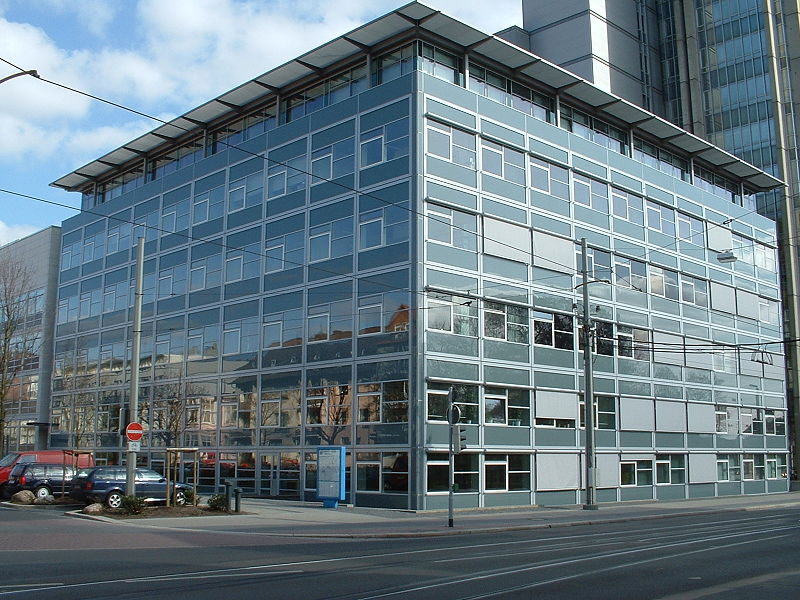
\includegraphics[width=\@current@width,height=\@current@height]{infozentrum}
  \end{lrbox}
% Definiere und platziere Textblock mit gespeichertem Inhalt.
  \ifthenelse{\boolean{tubsbox@bottomsender}}{%
    \begin{textblock*}{\@current@width}(%
      -\tubspage@borderwidth+\tubs@sb@box@xpos,%
      -\tubspage@borderwidth+\tubs@sb@box@ypos)%
        \setlength\fboxsep{0mm}%
        \colorbox{tuWhite}{%
          \hspace{0.5\tubs@sb@padding}%
          \usebox{\tubs@sb@storebox}%
          \hspace{0.5\tubs@sb@padding}%
        }%
    \end{textblock*}%
  }{%
    \begin{textblock*}{\@current@width}(%
      -\tubspage@borderwidth+\tubs@sb@box@xpos,%
      -\tubspage@borderwidth+0.05195\paperheight+\tubs@sb@box@ypos)%
        \setlength\fboxsep{0mm}%
        \tubsbox@framebox{\tubsbox@colorbox{%
          \usebox{\tubs@sb@bgimagebox}%
        }}%
    \end{textblock*}%
    \begin{textblock*}{\@current@width}(%
      -\tubspage@borderwidth+\tubs@sb@box@xpos,%
      -\tubspage@borderwidth+0.05195\paperheight+\tubs@sb@box@ypos)%
        \setlength\fboxsep{0mm}%
        \tubsbox@framebox{\tubsbox@colorbox{%
          \hspace{0.5\tubs@sb@padding}%
          \usebox{\tubs@sb@storebox}%
          \hspace{0.5\tubs@sb@padding}%
        }}%
    \end{textblock*}%
  }
  % Prüfe, ob Zeile gesplittet werden soll (opt. Arg. != \relax)
  \ifthenelse{\equal{\@current@rowheight}{\relax}}{%
    \addtolength\tubs@sb@box@xpos{\@current@width+0.5\tubspage@borderwidth}%
  }{%
    \setlength\tubs@sb@box@rowheight{\@current@rowheight}
    \addtolength\tubs@sb@box@ypos{\@current@height+0.5\tubspage@borderwidth}%
    \addtolength\tubs@sb@box@splitrow{\@current@height+0.5\tubspage@borderwidth}%
    % Wenn Zeilenhöhe ausgefüllt, normal weiter machen...
    \ifthenelse{\lengthtest{\tubs@sb@box@splitrow > \tubs@sb@box@rowheight}}{%
      \addtolength\tubs@sb@box@xpos{\@current@width+0.5\tubspage@borderwidth}%
      \addtolength\tubs@sb@box@ypos{-\tubs@sb@box@splitrow}%
      \setlength\tubs@sb@box@splitrow{0mm}%
    }{}
  }
  % Wenn Zeile gefüllt ist, springen in nächste Zeile
  \ifthenelse{\lengthtest{\tubs@sb@box@xpos > \textwidth}}{%
    \addtolength\tubs@sb@box@ypos{\@current@rowheight+0.5\tubspage@borderwidth}%
    \setlength\tubs@sb@box@xpos{0mm}%
    % Wenn darüber hinaus Seite gefüllt ist, fange neue an!
    \ifthenelse{\lengthtest{\tubs@sb@box@ypos > \textheight}}{%
      \setlength\tubs@sb@box@ypos{0mm}%
    }{}
  }{}
  % speichere global!
  \global\tubs@sb@box@xpos=\tubs@sb@box@xpos%
  \global\tubs@sb@box@ypos=\tubs@sb@box@ypos%
  \global\tubs@sb@box@splitrow=\tubs@sb@box@splitrow%
}
% Umgebungsende
\let\end@scifibox\end@@scifibox
%
\newcommand\scifibox@setdefault@opts{%
  \setkeys{tubsbox.sty}{bgcolor=tuWhite}
}
%    \end{macrocode}
%
% Behandlung von erstem optionalen Argument (keyvals)
%    \begin{macrocode}
\def\@scifibox@oparam[#1]{%
  \setkeys*{tubsbox.sty}{#1}%
  \setkeys*{gaussbox}{#1}%
  \@@scifibox
}
%    \end{macrocode}
%
% Test nach erstem optionalen Argument (keyvals)
%    \begin{macrocode}
\def\@scifibox{%
  \@ifnextchar[{%
    \@scifibox@oparam%
  }{%
    \@@scifibox%
  }%
}
%    \end{macrocode}
%    \end{macro}
%
%    \begin{macrocode}
%</package>
%    \end{macrocode}
%
% \Finale
\endinput
%
% Präfixe:
% tubs  - allgemeiner Präfix
% gb    - Präfix für gaussbox
% sb    - Präfix für scifibox
%